 \documentclass{article}
\usepackage{setspace}
\usepackage[hidelinks]{hyperref}
\usepackage{url}
\usepackage[utf8]{inputenc}
\usepackage[english]{babel}
\usepackage[a4paper,top=3cm,bottom=2cm,left=3cm,right=3cm,marginparwidth=1.75cm]{geometry}
\usepackage[T1]{fontenc}
\usepackage{graphicx}
\usepackage{longtable} %
\usepackage[caption = false]{subfig}
\usepackage{amsmath}
\usepackage{float}
\usepackage[style=authoryear,backend=biber]{biblatex}
\usepackage{lineno}
%\bibliographystyle{agsm}
%\usepackage{natbib}
\usepackage{csquotes}% Recommended
\doublespacing
\newcommand{\HRule}{\rule{\linewidth}{1mm}}
\addbibresource{main.bib}% Syntax for version >= 1.2
%\bibliography{main.bib}
%
\begin{document}
% title
\title{Functional Response Models and Consumer Temperature}%
\author{Ruth Keane}

\begin{titlepage}

\includegraphics[width=8cm]{logo.eps}\\[1cm] 
\center 
\textsc{\LARGE CMEE Miniproject}\\[1.5cm] 
\textsc{\Large Imperial College London}\\[0.5cm]
\textsc{\large Life Sciences}\\[0.5cm] 
\makeatletter
\HRule \\[0.4cm]
{ \huge \bfseries \@title}\\[0.4cm] % Title of your document
\HRule \\[1.5cm]
\makeatother
\Large \emph{Author:}\\
Ruth Keane \\[3cm] % Your name
\input{../Results/Tables/wordcount.txt}\\
{\large \today}\\[2cm] % Date, change the \today to a set date if you want to be precise
\vfill % Fill the rest of the page with whitespace
\clearpage
\end{titlepage}
\tableofcontents
\newpage
\linenumbers
\begin{abstract}
Functional responses of predators are effected by temperature and these relationships can be complicated. The nature of these relationships can have important implications for understanding interactions, particularly due to climate change. Three Holling models and two polynomial models were successfully fit to $241$ datasets containing functional response data. The best model for each dataset was analysed and compared at different temperature ranges. The search rate and handling times were also compared with temperature. The mechanistic Holling type II model was the most successful model  and the number of times each model was the best was significantly different from a uniform distribution but there was not a significant difference between mechanistic and phenomenological models. Temperature did not affect which Holling model was most successful but did affect whether phenomenological or mechanistic models were more successful, mostly due a polynomial model of degree three being very successful at $20-25$ degrees, which is likely due to the quality of the data at these temperatures. Log of search rate was weakly negatively correlated  to consumer temperature and log of handling time was weakly positively correlated with consumer temperature which was contrary to existing literature. This is probably because existing literature looks at temperature change within predator prey systems but in this case systems with different consumer temperatures were compared. 
\end{abstract}
\section{Introduction}
\subsection{Functional Responses and existing models}
The functional response describes how predators respond to changes in prey density (\cite{hollingsawfly1959,Solomon1949}). As prey numbers increase, the consumption rate of predators initially increases then levels out, however the specific shape of the period of increase can vary (\cite{hollingsawfly1959}). Holling modelled the functional response and suggested three different forms which he proposed worked for different types of organisms (\cite{hollingsawfly1959}). These are Type I, where the rate of increase in prey consumption with prey density is constant before a plateau, type I, where the rate of increase in prey consumption with prey density is decreasing (i.e the curve is hyperbolic (\cite{Jeschke2002PredatorPrey})) and type III, where the  rate of increase in prey consumption with prey density increases then decreases (\cite{hollingsawfly1959}). The type I model can be described by equation \ref{type1}, the type II model can be described by equation \ref{type2} where $x_R$ is the resource density, $c$ is the number of prey consumed per predator per unit time, $a$ is the discovery or search rate of the consumer and $h$ is the handling time (\cite{Dawes2013,Holling1959}). The type III model can be described by a generalised version of equation \ref{type2}, equation \ref{type3} where $q$ changes the shape of the curve (\cite{Dawes2013}). This is due to reduced predator efficiency when predator densities are low, so at lower densities prey mortality is decreased (\cite{Taylor2003EffectAmericanus,Hassell1978TheSystems.}). 
When $q=0$, the model is type II and when $q>0$,the model is type III (\cite{Dawes2013}). \\
\begin{equation}\label{type1}
    c=ax_R
\end{equation}
\begin{equation}\label{type2}
c=\frac{ax_R}{1+hax_R}
\end{equation}
\begin{equation}\label{type3}
c=\frac{ax_R^{q+1}}{1+hax_R^{q+1}}
\end{equation}

It is important to note that both the search rate and handling times are functions of different aspects of attacking and eating prey (\cite{Hassel1976TheDeath-Rate}). The handling time is made up of the time predators spend pursuing, subduing, eating and digesting their prey. The search rate (or discovery rate) combines the distance at which a predator will attack prey, the speed of both the prey and the predator and the success rate of attacks (\cite{Holling1966}). In general, the Holling type II model is very successful, especially considering its simplicity, however there are examples where data is better described by a more complex model, such as a type III Holling model (\cite{Hassel1976TheDeath-Rate}) . 
Many other models exist to describe the functional response, often based on variations of the Holling equation accounting for different behavioural aspects  (\cite{Jeschke2002PredatorPrey}). \cite{Jeschke2002PredatorPrey} attempted to separate handling and digestion time from  $h$.  If values of $a$ or $h$ change with prey density, then the Holling II model may not fit well  (as $a$ and $h$ are constant in this model). In these examples, the type III Holling model can be a good model (\cite{Hassel1976TheDeath-Rate}). 
\subsection{Temperature and Functional Responses}
Many biological traits are dependent on temperature (\cite{Dell2014TemperatureStrategy,Dell2011SystematicTraits}), in particular, the body velocity(\cite{Dell2014TemperatureStrategy}). The way in which traits vary with temperature can depend on many factors including life stage (\cite{Cator2019MoreResearch}), habitat (\cite{Dell2011SystematicTraits}) and thermy (\cite{Dell2014TemperatureStrategy}). In addition often there is asymmetry between predator and prey response to temperature (\cite{Dell2014TemperatureStrategy}). This means that understanding how the functional response of predators changes with temperature can be very complicated. The functional response of predators has important applications in nature and agriculture (for example in biological control of agricultural pests (\cite{Gilioli2005TemperatureIndividuals})). The response of the functional response to changes in temperature is important in predicting the effect of climate change (\cite{Ohlund2014TemperaturePrey}).  \\
The metabolic theory of ecology (\cite{Brown2004TowardEcology}) predicts that handling time reduces exponentially and search rate increases exponentially when temperature is increased (\cite{Dell2014TemperatureStrategy}). Increases in search rate when temperature is increased have been found in multiple predator-prey systems(\cite{Gilioli2005TemperatureIndividuals,Zamani2006Temperature-dependentAphid}). Many studies have found that this increases reaches a plateau or decreases after a maximum (\cite{Thompson1978TowardsElegans,Zamani2006Temperature-dependentAphid,Sentis2012UsingEfficiency}). Experimentally changing the temperature in predator prey systems does reduce the handling time(\cite{Thompson1978TowardsElegans,McCoull1998EffectNaucoridae,Jalali2010EffectPersicae,Zamani2006Temperature-dependentAphid}), sometimes exponentially (\cite{Sentis2012UsingEfficiency,}). \\
The response between type of functional response and temperature is less clear. Some studies have found no effect of temperature on type of functional response  (\cite{Sentis2012UsingEfficiency}) but there are examples of the functional response changing with temperature (\cite{Taylor2003EffectAmericanus}).
\subsection{Model Types}
Models can be phenomenological or mechanistic. In mechanistic models, all parameters have biological meaning and in phenomenological models they do not; instead a function is used that fits the data or processes (\cite{Otto2007AEvolution,Geritz2012MathematicalModels}). Phenomenological models may fit better to data and can be very useful in the absence of mechanistic models. They can be easier to understand, however do not have as much biological meaning as mechanistic models (\cite{Otto2007AEvolution}). \cite{Geritz2012MathematicalModels} claim that this could stop them being valid for use in biological systems.  
Mechanistic models can improve our understanding of biology and are useful for making predictions more accurately because when the meanings of parameters of known, biological constraints can be included. Although they are simplifications of systems and may have strong assumptions, they can improve biological understanding and can include as much information about the system as is available (\cite{Otto2007AEvolution,Kendall1999WhyApproaches}). How well a simplified model fits to data can give important insight into what aspects of a system are important in determining the dynamics (\cite{Geritz2012MathematicalModels}).
The Holling models described above are mostly mechanistic but the type III model is more phenomenological due to the non-biological parameter $q$. Even the Holling type II model may be partially phenomenological because the values of $a$ and $h$ are a functions of  multiple biological components (\cite{Hassel1976TheDeath-Rate}).
\subsection{This work}
In this paper, five models were fitted to experimental functional response data: Holling's type I-III and polynomials of degree two (to capture increasing and levelling out of the functional response) and three (to capture a change in the rate of increase of the functional response). Then the best model for each experiment was determined from the lowest AIC. The Holling II model was predicted to be the best model. It was expected that the Holling type III model would be able to fit better to the data but may have a higher AIC value due the the extra parameter.  The best model was found at different consumer temperature ranges to explore whether this led to different models fitting better. In addition the search rate and handling times from the Holling's models were compared to the consumer temperature to explore whether functional response parameters for systems with different consumer temperatures would show similar responses to the studies looking at different temperatures within the same system. It was expected that search rate would increase with temperature, then reach a maximum and decrease. It was expected that handling time would decrease with temperature.

\section{Methods}
\subsection{Computing Tools}
Bash was used to compile the pdf of the tex file, to calculate and format the word count of the project (using teXcount) and to run the project files. This was used due to the ease of accessing files and files contents in bash. In addition, bash can easily run other programs.
Python (with pandas, numpy and csv) was used to sort the data, add new columns to the dataset and remove datasets with an insufficient number of points and export this updated dataframe as a csv. These tasks are well suited to Python's abilities.
R was used to fit models, plot graphs and analyse data due to the versatility of its dataframe structures. In addition plotting in ggplot2 is very flexible. "xtable" in R was used to  integrate tabular results from R in tex files. "minpack.lm" in R was used to fit Holling models using Levenberg-Marquardt nonlinear least squares (\cite{Elzhov2016}).
\subsection{Initial Data Sorting}
The data used was from the Biotraits database (\cite{Dell2013}), which contains information collated from different studies about how biological traits respond to environmental drivers including functional response data. The parameters of interest here were the number of prey the predator consumed per unit time and the resource density. Data sorting was carried out in python version 2.7. New columns were added and experiments with less than six experiments were removed. This new dataset was exported to a csv for model fitting.
\subsection{Model Fitting}
The data were fitted to five different models: a quadratic model, a cubic model and the three Holling models (\cite{Holling1959}) using R 3.6.2 (\cite{RCoreTeam2017}). The Holling models were type I  (equation \ref{type1}, a linear model where the intercept was the origin), type II  (equation \ref{type2}) and generalised type III (equation \ref{type3}). Models were fitted sequentially for each experiment and plotted. This allowed the fit to be visually inspected as the model fitting process was improved.
\subsubsection{Fitting Linear models}
 The Holling type I, quadratic and cubic models models were fitted using lm (base R). For the quadratic and cubic models, poly was used to compute orthogonal polynomials to avoid correlation of variables.
\subsubsection{Fitting Non-linear Models}
The Holling type II and type III models were fitted using NLSlm (from the package minpack.lm (\cite{Elzhov2016}). The coefficients $a$, $h$, and $q$ were given a lower bound of zero and the maximum number of iterations was set to $1000$. For both type II and type III models, starting values were calculated using starting value functions where $a$ and $h$ were estimated. The initial value for $h$ was the maximum value of $c$. The initial value for $a$ was the initial steepest part of the curve which was calculated by repeatedly fitting linear models to the dataset then deleting the maximum value of $x_R$ and storing the largest gradient of these models. For the type III model, this initial value of $q$ was picked from a random uniform distribution between -2 and 2. Finding the starting values was followed by sampling positive values around these initial values, repeatedly running the models and storing the coefficients and AIC values of these models. The coefficients of the model with the lowest AIC were used as the initial values for the main model fitting step. Once the starting values had been determined, the models were rerun with these initial values. 
\subsection{Data Analysis}
Data analysis was carried out in R 3.6.2(\cite{RCoreTeam2017}).The models were compared using AIC and the most appropriate model was determined for each dataset. AIC was used because other techniques to compare models are not appropriate for non linear models. Between AIC and BIC, AIC was used because it penalises extra parameters more at lower sample sizes than BIC (\cite{Johnson2004ModelEvolution}). As this dataset contains  a number of experiments with small sample sizes, this could prevent an overfitted model being selected as the best model.\\ 
The confidence intervals for values of $q$ were calculated (from the mean $\pm2SE$, where $SE$ is the standard error). When the confidence interval for $q$ overlapped zero, the best AIC was recalculated for the remaining Holling models (because when the confidence interval for $q$ is zero, the type III model is the same as the type III model).
A chi-square ($\chi^2$) goodness of fit test was carried out on the best model and the best model type (phenomenological or mechanistic) to determine if the number of models in each category was significantly different.\\
The p-value of each parameter for each model was stored and if it was not significant, the parameter was removed from analysis. The log consumer temperatures and log parameter were not normally distributed and there ties in the data so Spearman's rank correlation could not be calculated.  Kendall rank order correlation tests were carried out on consumer temperatures and log search rate and consumer temperatures and log handling time for each of the Holling models. Log of the parameters was used because both search rate and the handling time values were mostly very low with  a few very large values. The search rate for type III models could not be tested due to a low number of models were search rate was significant. \\ 
Chi-square ($\chi^2$) tests were carried out to determine the association between consumer temperature and best model type and consumer temperature and best Holling model (recalculated). The temperature values were discretised by creating an expectation table with intervals of five degrees and combining these intervals until the expected values were all greater than five.
\section{Results}
\subsection{Number of Fits}
Many of the models fit well to the data, for example (Figure\ref{fig:2}). Most models successfully fit the data. Of the 241 datasets, only $\input{../Results/Tables/failII}$ Holling type II models and $\input{../Results/Tables/failIII}$ Holling type II models did not converge. 
\begin{figure}[h!t] 
    \centering
    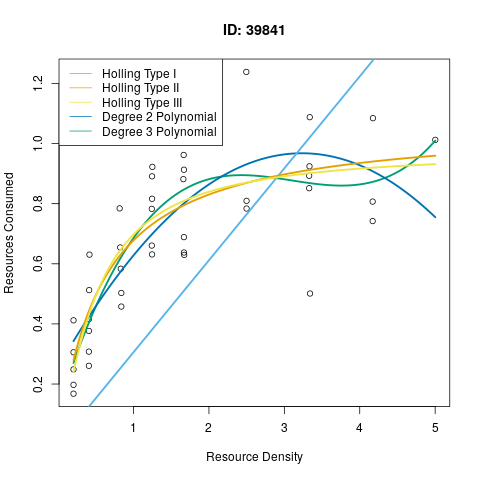
\includegraphics[width=2.3in]{../Results/Plots/39841.png}
    \caption{This is a graph for the experiment with ID 39841}
    \label{fig:2}
\end{figure}
\subsection{Best Model}
The Holling's type II model was most frequently the best model ($\input{../Results/Tables/holIIbest}\%$) and the polynomial of degree 2 was most frequently the second best model ($\input{../Results/Tables/poly32best}\%$) (Figure \ref{fig:bestmodel}).
The mechanistic models were marginally more often the best model ($\input{../Results/Tables/mechbest}\%$)than the phenomenological models (Figure \ref{fig:modelbesttype}).
\begin{figure}[ht!]
\centering
\subfloat[Number of times that each model was the best model]{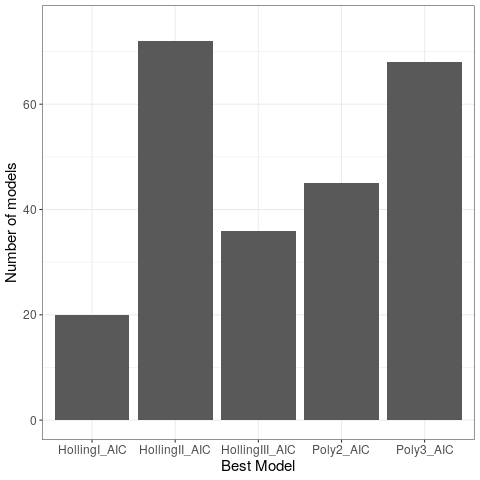
\includegraphics[width = 3in]{../Results/Plots/modelbest.png}}
\subfloat[Number of times that each model was the second best model]{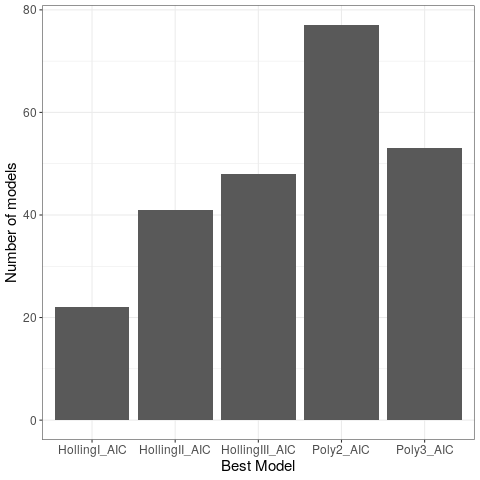
\includegraphics[width = 3in]{../Results/Plots/modelsecondbest.png}}
\caption{Best and second best model from the lowest and second lowest AIC values. Models are Holling type I, Holling type II, Holling type II, polynomial of degree 2, polynomial of degree 3. $n=241$}
\label{fig:bestmodel}
\end{figure}
\begin{figure}[h!t] 
    \centering
    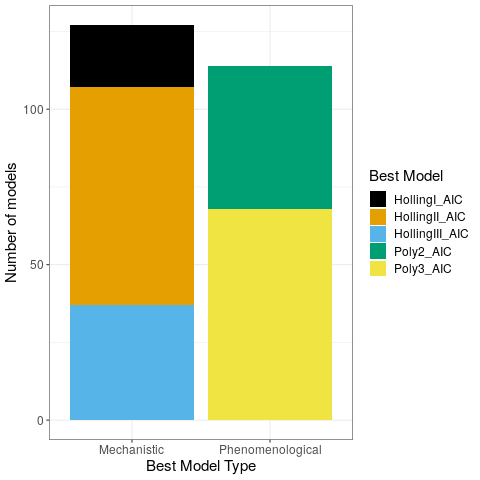
\includegraphics[width=4in]{../Results/Plots/modelbesttype.png}
    \caption{Number of models where the best type was phenomenological or mechanistic. Colour is the model. $n=241$}
    \label{fig:modelbesttype}
\end{figure}
The distribution of the best model was not best described by a uniform distribution ($p<0.05$,Table\ref{chitable}).  The distribution of the best model type was best described by a uniform distribution (p>0.05,Table\ref{chitable}).
\input{../Results/Tables/output_chitable_latex.txt}
\subsection{Best Holling Model}
Of the three Holling models, the type II model was the best (Figure\ref{fig:bestholandrecalmodel}). The best Holling model was recalculated, removing the type III Holling model when the confidence interval for $q$ spanned $0$ ($\input{../Results/Tables/recaldiff}$ models). The majority of these were best described by the Holling type II model of the other Holling models, but some were better described by the type I model (Figure \ref{fig:bestholandrecalmodel})
\begin{figure}[h!]
\centering
\subfloat[Number of times that each model was the best  Holling model]{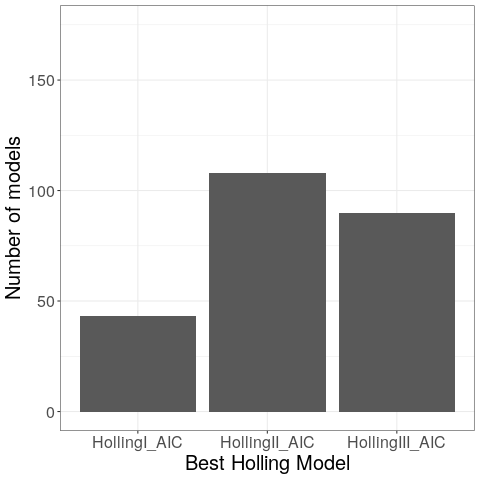
\includegraphics[width = 2in]{../Results/Plots/modelbestholl.png}}
\subfloat[Number of times that each model was the best Holling model, when the best Holling model was recalculated]{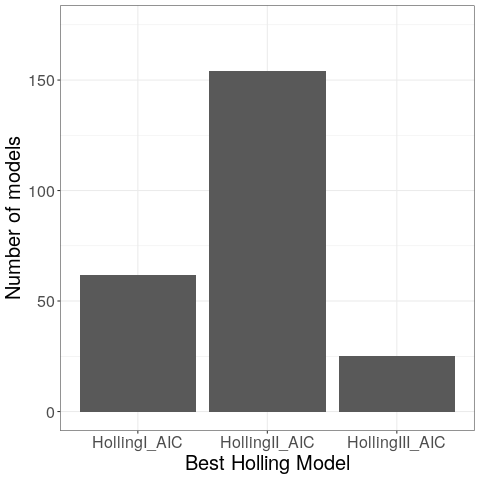
\includegraphics[width = 2in]{../Results/Plots/modelbesthollrecal.png}}
\caption{Best model from the lowest AIC values (of the Holling model). Models are Holling type I, Holling type II and Holling type II. $n=241$}
\label{fig:bestholandrecalmodel}
\end{figure}
\subsection{Temperature and Best Model}
The type of the best Holling model did not vary much with the temperature (Figure \ref{fig:tempholandmodel}) and the temperature interval was not associated with the best Holling model.($\chi^2=\input{../Results/Tables/chiholrtemp}$,$p=\input{../Results/Tables/pholrtemp}$,$df=\input{../Results/Tables/dfholrtemp}$). At most temperatures ($<20$ degrees), more mechanistic models fit the best better . However at the interval $20-25$ degrees, more phenomenological models fit the best (Figure \ref{fig:tempholandmodel}).  The temperature interval was associated with the best model type ($\chi^2=\input{../Results/Tables/chitypetemp}$,$p=\input{../Results/Tables/ptypetemp}$,$df=\input{../Results/Tables/dftypetemp}$). This difference seemed to be due to the polynomial of degree three being particularly successful in the interval $20-25$ degrees.
\begin{figure}[h!]
\centering
\subfloat[Number of times a mechanistic or a phenomenological model was the best model at each consumer temperature interval.]{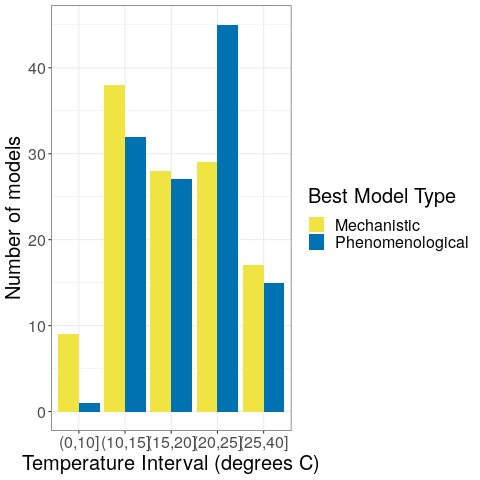
\includegraphics[width = 2in]{../Results/Plots/temppmodeltype.png}}
\subfloat[Number of times the recalculated Holling model was the best model at each consumer temperature interval. ]{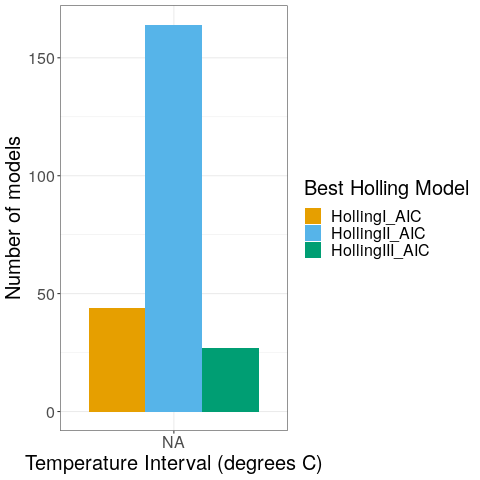
\includegraphics[width =2in]{../Results/Plots/tempmodelrhol.png}}\\
\subfloat[Number of times each model was the best model at each consumer temperature interval.]{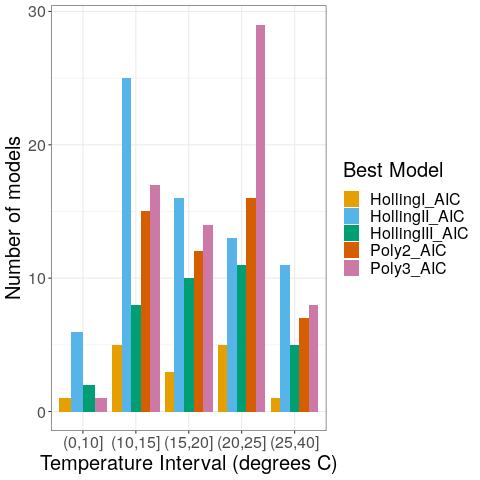
\includegraphics[width = 3.5in]{../Results/Plots/tempmodel.png}}
\caption{Best model is determined from the lowest AIC values.  Colour is the best model type. $n=241$}
\label{fig:tempholandmodel}
\end{figure}
\newpage
\subsection{Temperature and Parameter Values}
The consumer temperatures are  weakly negatively correlated with the search rate for type I and type II Holling models (Figure \ref{fig:tempparam},Table \ref{Paramtemp}).The search rate is smaller and less varied at intermediate temperatures, however at very low and very high temperatures, the temperature is very varied and can be very high. The consumer temperatures are weakly positively correlated with handling time for type II and type III Holling models (Figure \ref{fig:tempparam},Table \ref{Paramtemp}).
\input{../Results/Tables/output_temp_con_latex.txt}
\begin{figure}[h!t]
\centering
\subfloat[Consumer temperature and log search rate for type I Holling model]{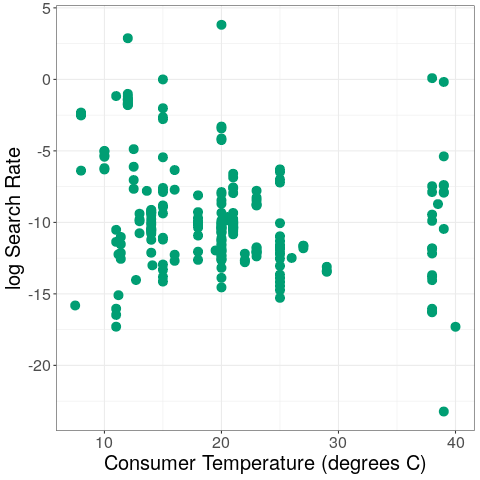
\includegraphics[width = 2.5in]{../Results/Plots/plot1conA.png}}\\
\subfloat[Consumer temperature with log search rate for type II Holling model]{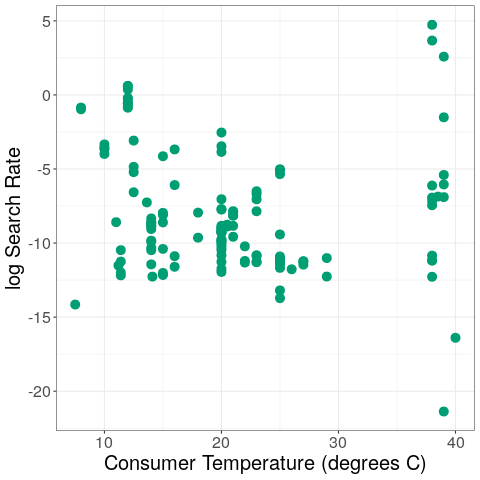
\includegraphics[width = 2.5in]{../Results/Plots/plot2conA.png}}
\subfloat[Consumer temperature with log handling time for type II Holling model]{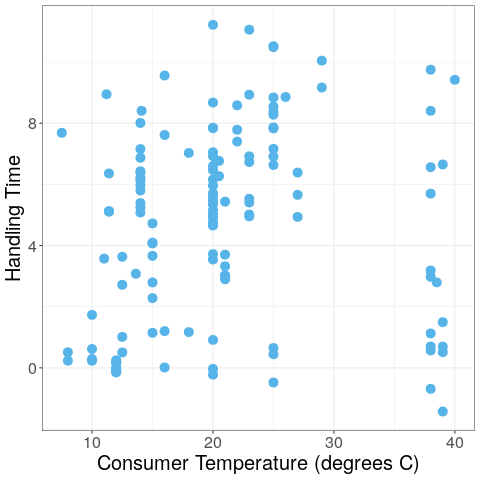
\includegraphics[width = 2.5in]{../Results/Plots/plot2conH.png}} \\
\subfloat[Resource temperature with log search rate for type III Holling model]{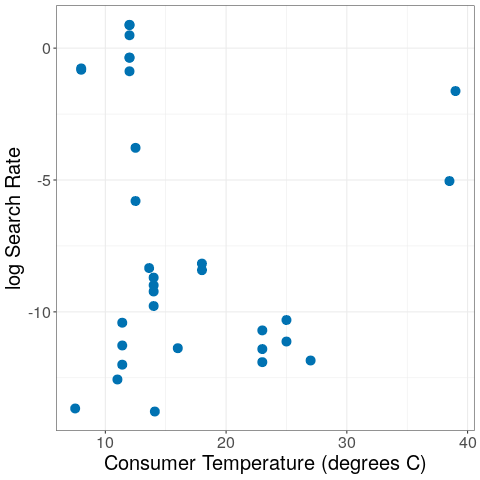
\includegraphics[width = 2.5in]{../Results/Plots/plot3conA.png}}
\subfloat[Consumer temperature with log handling time for type III Holling model]{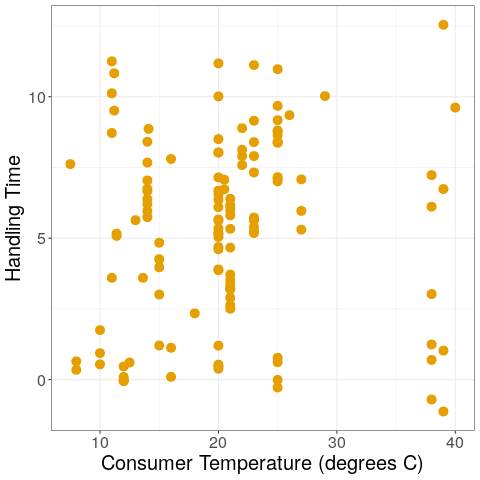
\includegraphics[width = 2.5in]{../Results/Plots/plot3conH.png}}
\caption{Logged parameter values and Consumer temperature for Type I, Type II and Type II Holling Models.}
\label{fig:tempparam}
\end{figure}
\clearpage
\section{Discussion}
\subsection{Holling Model Recalculated}
Initially the Holling type II model was the most successful model, followed by the Holling type III model, then the Holling type I model (Figure \ref{fig:bestholandrecalmodel}). This was expected from the literature as type II models are very common, type I responses are limited to filter feeders (\cite{Jeschke2004Consumer-foodFeeders}) and type III responses are frequently seen, for example in \textit{Daphnia} (\cite{Sarnelle2008TypeDaphnia}). There was not sufficient time to explore what type of organisms had each type of functional response but it is likely given existing knowledge that the systems showing type I responses are filter feeders (\cite{Jeschke2004Consumer-foodFeeders}). Recalculating the best model so that Holling type III was the best model only when $q$ was significantly different from $0$ meant that the type I Holling model became more successful than the Holling type III model. This response was contrary to existing knowledge about functional responses, for example \cite{Dunn2020PredatorHabitats} found a proportion of each model similar to the initial proportion of the best functional response type. It is possible that the initial result overestimated the number of experiments showing type III responses because it doesn't take into account the value of $q$, which could be very close to $0$ (equivalent to a type II response). The method of recalculating the best model could be improved to ensure that datasets showing a true type III response are not removed. This could be achieved by taking the units of $x_R$ and $c$ into account. Alternatively, the dataset could be biased towards type I functional responses models because they include organisms that may be easier to study than non-filter feeders(\cite{Jeschke2004Consumer-foodFeeders}).
\\
As for the phenomenological models, the polynomial of degree three best described the data almost as frequently as the type II models \ref{fig:bestmodel}. It is possible that this could indicate a type III functional response (fitting better to a phenomenological model than a mechanistic model). Alternatively the type III model could be capturing decreases in consumption at high prey densities, which is seen in some datasets. It was not possible to control where the point of inflection was, so this model is likely to capture patterns not caused by type III responses. The polynomial of degree two could capture the increase in resource consumption followed by plateau (where the plateau is the maximum of the peak of the polynomial). It was somewhat successful, however not as successful as the Holling type II model. It was most frequently the second best model which could be indicating that is successfully capturing the type II responses, albeit not as effectively a Holling's type II model. This could be because it has one more parameter than the Holling model, which is penalised by the AIC. Alternatively, the polynomial might fit less well to type II responses because the polynomial curve decreases after maximum instead of levelling out as is seen in Holling type II responses. 
\subsection{Mechanistic and Phenomenological }
In general mechanistic models performed slightly better than phenomenological models but this difference was not significant. It is not unexpected that phenomenological models fit the data well but it may not be biologically useful. Phenomenological models can fit well to any dataset, so are more likely to fit to poor quality data or data, which may be the reason they were successful. Additionally, their flexibility may lead to graph shapes that are not biologically feasible. This means the examples where the polynomial phenomenological models fit better to data may have less biological meaning, and should not be interpreted as showing a type II or type III phenomenological responses unless the plot or coefficients are examined in more detail. Phenomenological models may fit better to data showing relationships not predicted by the mechanistic models. This may indicate a possibility for improving the mechanistic models and acquiring a more biological understanding of this aspect of the relationship, which could be scope for future study
\subsection{Temperature}
The origin of the temperatures is likely to have varied between datasets. If the consumer temperature was missing, the ambient temperature was used instead. Additionally, the dataset contained both ectotherms and endotherms which have very different body temperatures and respond very differently to temperature changes. Ectotherms are more effected by changes in temperature (\cite{Dell2014TemperatureStrategy}).
\subsubsection{Temperature and Model}
Temperature did not affect the type of the Holling model however it did have a significant impact on whether the best model was phenomenological or mechanistic \ref{fig:tempholandmodel}.  Although Holling type does vary with temperature in some systems, for example in shrimp and flounder (\cite{Taylor2003EffectAmericanus}), there is not evidence in the literature for this occurring between systems. This is due to the success of the polynomial of degree two and three varying with temperature. At $0-10$ degrees, the polynomial of degree  two was never the best model and the polynomial of degree three was only the best model once. At $20-25$ degrees, the polynomial of degree three and two were the two best models respectively.  From examining the plots, in this temperature interval, there were many models with few different resource densities, sometimes due to repeats. To make results more accurate to biological reality, the minimum number of datapoints for a dataset to be used could be reduced and the number of unique resource densities could be taken into account.
\subsubsection{Handling Time and Search Rate}
Log search rate was negatively correlated with temperature, which is in contrast with what is seen in the literature(\cite{Thompson1978TowardsElegans,Zamani2006Temperature-dependentAphid,Sentis2012UsingEfficiency,Gilioli2005TemperatureIndividuals,Dell2014TemperatureStrategy,Englund2011TemperatureResponse}). Log handling time was positively correlated with temperature which also contrasts with the literature (\cite{Dell2014TemperatureStrategy,Thompson1978TowardsElegans,McCoull1998EffectNaucoridae,Jalali2010EffectPersicae,Zamani2006Temperature-dependentAphid,Sentis2012UsingEfficiency}).  
These differences could be due to temperature related adaptations of the organisms in these studies. At warmer temperatures, the risk of overheating could select for slower movement so larger search rates and longer. It should be noted that Kendall's rank order correlation is prone to false positives when $n$ is large (\cite{Dytham2011ChoosingEdition}) so it is possible that there is no correlation between the temperature and the search rate or handling time.
In much of the literature, temperature changes within predator-prey systems are compared. However,here, temperatures between different predatory-prey systems were compared so this finding is completely in constrast to previous work. 
It is possible that combining ectotherm-ectotherm, endotherm-ecotherm and endotherm-endotherm systems is the reason for unexpected results as the type of system is likely to effect search rate and handling time (\cite{Dell2014TemperatureStrategy}). In future analysis could be repeated separately for these systems, however the dataset does not contain a large number of endotherms so this is unlikely to have a large effect. Similarly, the habitat is likely to effect this relationship (\cite{Dell2014TemperatureStrategy}). Comparing search rate and handling time becomes very complicated when comparing vastly different systems. 
 \\
 \section{Conclusion}
In conclusion, the Holling type II model fit most of the models best and mechanistic models were slightly better than phenomenological models. The temperature affected the search rate and handling time in unexpected ways which is most likely due to the complexity of the data studied but could be due to adaptation to different temperatures.

\clearpage{}

\printbibliography
\end{document}

